\section{Esempi d’uso}
% Show how to use the produced software artefacts.

% Ideally, there should be at least one example for each scenario proposed above.

Come gi\'a descritto, il sistema permette l'utilizzo di due tipologie di utenti: User e Admin. In quanto non richiesto e non importante ai fini dell'esame, l'avvio del client nelle due modalit\'a \'e effettuato semplicemente tramite il passaggio o meno del flag "admin" alla funzione di avvio \textit{main}. Ci\'o \'e possibile sia tramite l'utilizzo di un ide, sia tramite il comando gradle \texttt{start\_client -Padmin} (richiede che il main container sia gi\'a in esecuzione).\\
L'interfaccia grafica non \'e stata studiata per essere responsiva ed \'e possibile riscontrare blocchi in attesa, ad esempio, della ricerca degli agenti nel \textit{DirectoryFacilitator}. Inoltre, possibili failure come errori di rete sono visibili solo tramite l'analisi della riga di comando e dunque non visibili dall'interfaccia. Tutte queste semplificazioni alla GUI sono state effettuate in modo da concentrarsi principalmente sullo sviluppo dell'infrastruttura ad agenti senza perdere tempo nell'implementazione di funzionalit\'a grafiche di poco conto.

\subsection{User}
Relativamente all'User, i casi d'uso principali sono:
\begin{enumerate}
    \item sottomissione di un ordine
    \item visualizzazione dello stato degli ordini passati
\end{enumerate}
L'interfaccia si avvia sulla schermata dello shop, dalla quale \'e possibile selezionare gli \textit{items} richiesti e piazzare un ordine (vedasi Figura \ref{fig:application-shop}).
\begin{figure}[!ht]\centering
    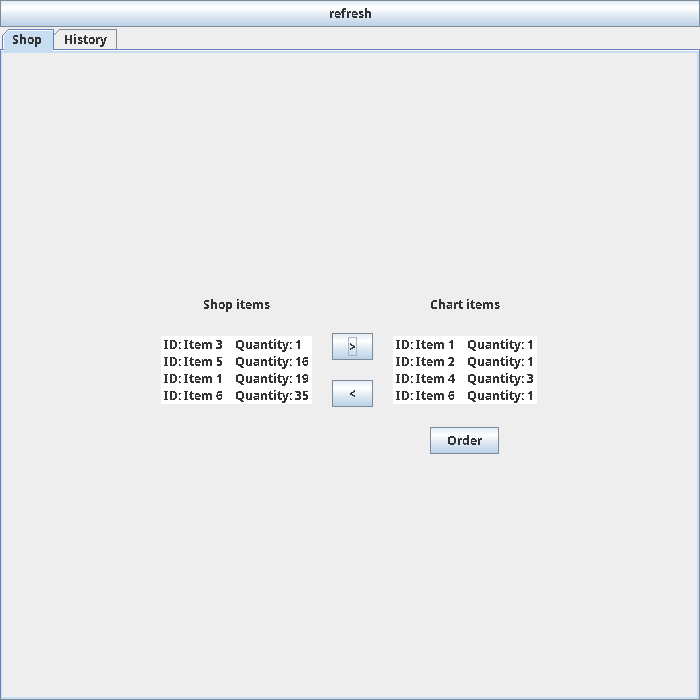
\includegraphics[width=.75\textwidth]{section/usage_examples/figure/application-shop.png}
    \caption{Interfaccia User per la sottomissione di ordini.}
    \label{fig:application-shop}
\end{figure}
L'ordine \'e poi preso in carico dall'\textit{order\_manager}, il quale far\'a partire la procedura di completamento degli ordini. \'E possibile visualizzare lo stato di quest'ultima nella schermata dello storico ordini (vedasi Figura \ref{fig:application-history}).
\begin{figure}[!ht]\centering
    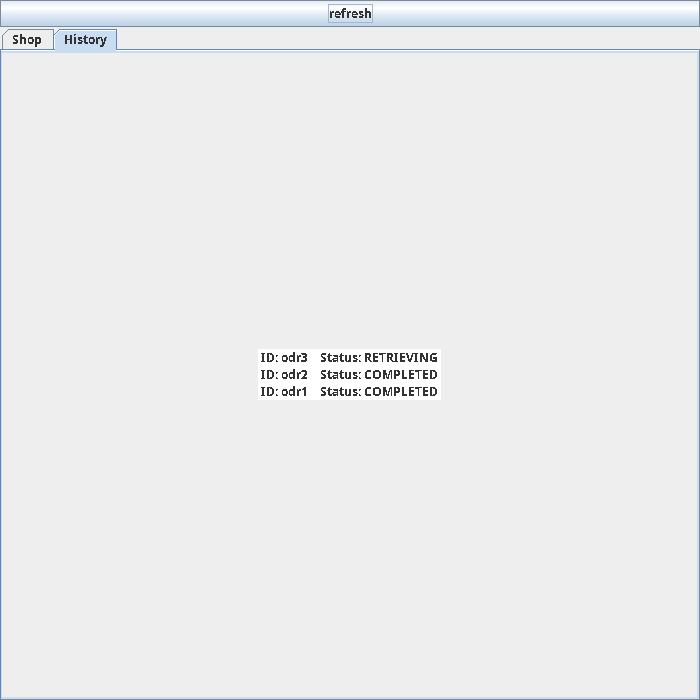
\includegraphics[width=.75\textwidth]{section/usage_examples/figure/application-history.png}
    \caption{Interfaccia User per il controllo degli stati degli ordini.}
    \label{fig:application-history}
\end{figure}

Non trattandosi di un processo automatico, la pressione del pulsante refresh \'e infine necessaria per l'aggiornamento dei dati nella schermata.

\subsection{Admin}
Relativamente all'Admin, i casi d'uso principali sono:
\begin{enumerate}
    \item visualizzazione dello stato del magazzino
    \item aggiunta e rimozione di \textit{items}
    \item visualizzazione dello stato del \textit{repository} di comandi
    \item aggiunta di un comando al \textit{repository}
    \item richiesta di esecuzione del comando da parte di un agente del sistema preposto allo scopo (allo stato attuale, solo i robot)
\end{enumerate}
L'interfaccia si avvia sulla schermata del magazzino, dalla quale \'e possibile aggiungere, rimuovere e visualizzare la disposizione degli oggetti al suo interno (vedasi Figura \ref{fig:application-warehouse}).
\begin{figure}[!ht]\centering
    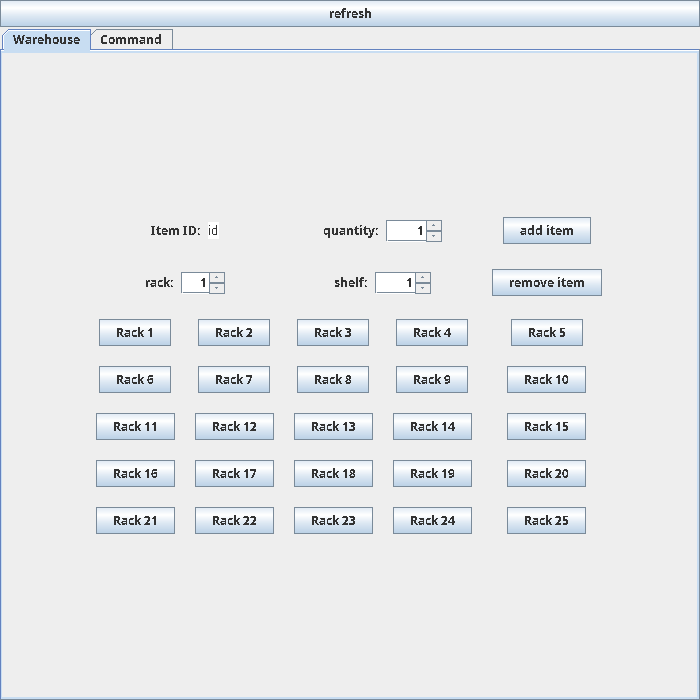
\includegraphics[width=.75\textwidth]{section/usage_examples/figure/application-warehouse.png}
    \caption{Interfaccia Admin per il controllo dello stato del magazzino.}
    \label{fig:application-warehouse}
\end{figure}
L'aggiunta permette di inserire un oggetto in uno slot che che sia vuoto o contenga un prodotto dello stesso tipo. La rimozione permette invece di rimuovere una specifica quantit\'a di un elemento senza per\'o la possibilit\'a di specificarne la posizione.
Cliccando su di un \textit{rack} \'e invece possibile visualizzare i prodotti in esso contenuti (vedasi Figura \ref{fig:application-rack}).
\begin{figure}[!ht]\centering
    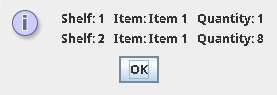
\includegraphics[width=.75\textwidth]{section/usage_examples/figure/application-rack.png}
    \caption{Dialog dell'interfaccia Admin per il controllo dello stato di un rack del magazzino.}
    \label{fig:application-rack}
\end{figure}

\parag
La schermata dei comandi (visibile in Figura \ref{fig:application-command}) permette la visualizzazione dei \textit{tasks} salvati e presenti nel \textit{repository} di piani; la loro modifica e successivo salvataggio; la possibilit\'a di richiederne l'esecuzione. Perch\'e un comando sia eseguibile \'e necessario che questo abbia i \textit{plans} che lo compongono preceduti da una label nella forma \texttt{@lN}, dove \texttt{N} rappresenta un indice incrementale che parte da 0. Questa `etichettatura' \'e necessaria per la corretta esecuzione dei piani ed in futuro potrebbe essere possibile applicarla in automatico allo \textit{script} sottomesso. Inoltre, per l'esecuzione \'e necessario che il piano sia stato precedentemente salvato nel \textit{repository}.
\begin{figure}[!ht]\centering
    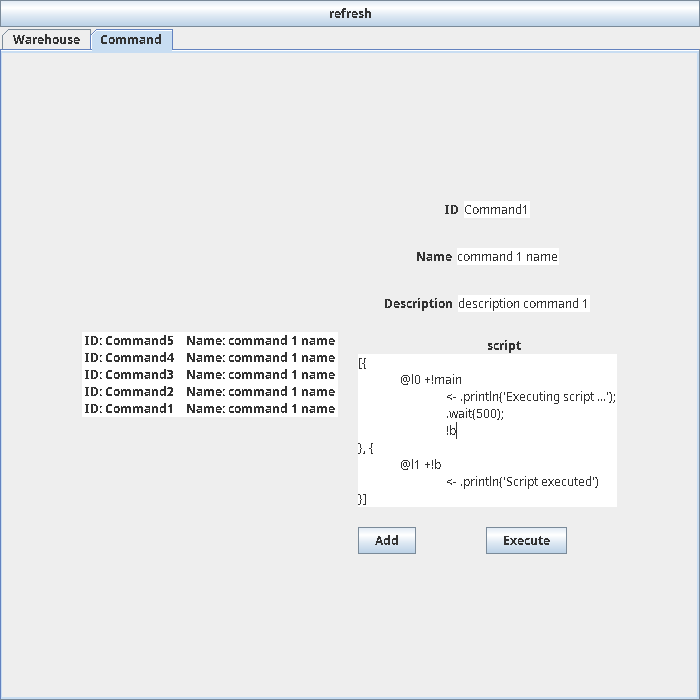
\includegraphics[width=.75\textwidth]{section/usage_examples/figure/application-command.png}
    \caption{Interfaccia Admin per il controllo dello stato del \textit{repository} di comandi.}
    \label{fig:application-command}
\end{figure}
